% Chapter Template

\chapter{模块设计} % Main chapter title

\label{Chapter3} % Change X to a consecutive number; for referencing this chapter elsewhere, use \ref{ChapterX}

\section{记录管理模块}
记录管理模块主要负责在数据库中创建、打开、删除一个数据表,在表中插入、删除、更新一条记录,以及遍历表找到所有符合条件的记录。

我们在项目中把每张数据表存在独立的文件中。文件均由页式文件系统管理,每个数据表文件的第一页是表文件头页,记录整个数据表的一些信息;之后的页均为数据页,每个数据页的页头记录该页的一些信息。

具体地,表文件头页按以下格式组织:
\begin{figure}[H]
\centering
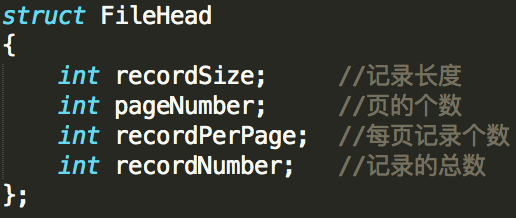
\includegraphics[width=3in]{Figures/FileHead.png}
\end{figure}
表文件头页中依次记4个整数,分别表示该表中记录长度、页的个数、每页的记录个数和表中记录总数。文件头页其余位置留空,可以用作其他扩展。

数据页每页8KB,前96 byte为页头,记录该页的一些信息,之后依次是固定长度的槽,每个槽可以放一条记录。数据页头按以下格式组织:
\begin{figure}[H]
\centering
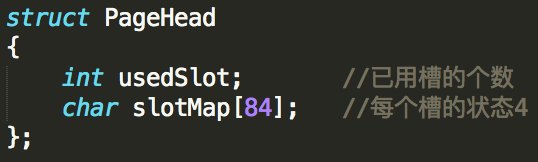
\includegraphics[width=3in]{Figures/PageHead.png}
\end{figure}
数据页头首先存放一个整数,记录本页已经放了几条记录。之后84 byte中每一个bit依次对应之后每个槽的状态,0表示为空,1表示已经有记录。

本模块的实现主要包括3个类,分别是RM\_Manager、RM\_FileHandle 以及 RM\_FileScan。在实现各个功能时,使用和维护之前所述的文件头、页头的信息。

\begin{figure}[H]
\centering
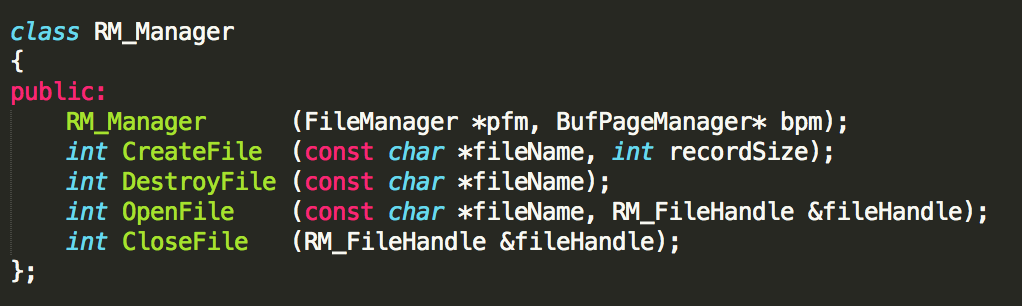
\includegraphics[width=5in]{Figures/RM_Manager.png}
\end{figure}

RM\_Manager提供的接口包括:(1)新建一个文件,生成表文件头页;(2)删除一个文件;(3)打开一个文件,得到一个RM\_FileHandle,可以通过其进行对记录的操作;(4)关闭一个文件。

\begin{figure}[H]
\centering
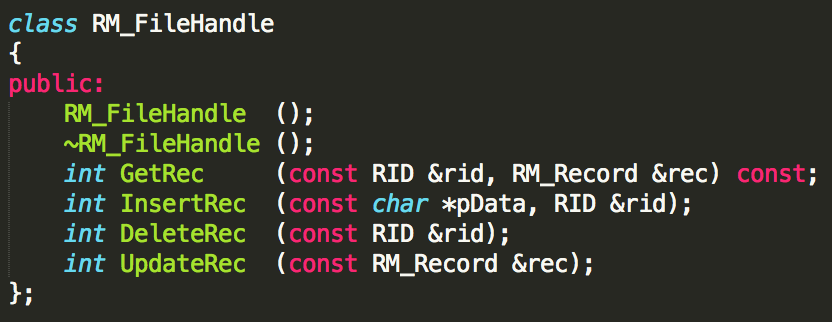
\includegraphics[width=4.5in]{Figures/RM_FileHandle.png}
\end{figure}

RM\_FileHandle提供的接口包括:(1)根据RID获得记录内容;(2)插入一条记录,返回位置标识RID;(3)根据RID删除一条记录;(4)更新一个记录(知晓RID)。

\begin{figure}[H]
\centering
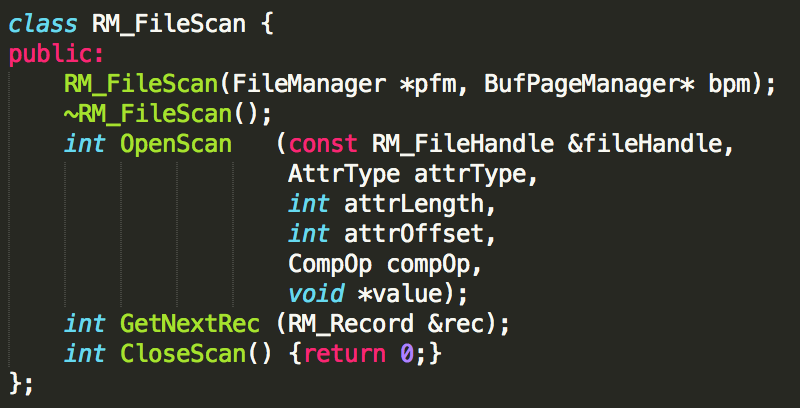
\includegraphics[width=4.2in]{Figures/RM_FileScan.png}
\end{figure}

RM\_FileScan提供的接口包括:(1)打开一个Scan,指定数据类型、长度、位置、约束条件;(2)获得一条符合条件的记录;(3)关闭一个Scan。

\section{系统管理模块}

\section{查询解析模块}

\section{索引模块}
索引模块的功能是为表中的某一属性建立索引,提高查询速度。

我们项目中索引使用B+树的数据结构实现,每个索引存放在一个独立的文件中。索引文件的命名方式是RelName.AttrName.index。索引文件由页式文件系统管理,有三种页,分别是索引文件头页、中间节点页、叶子节点页。

具体地,索引文件头页按以下方式组织:
\begin{figure}[H]
\centering
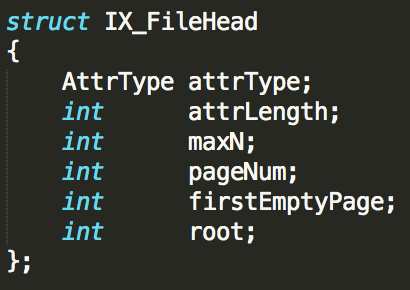
\includegraphics[width=2.5in]{Figures/IX_FileHead.png}
\end{figure}

 索引文件头页中记录索引数据的类型、长度、每页最多放多少索引项、已使用页的数量、根节点页等。

 之后的每个页页头也需要记录一些内容,包括
 \begin{figure}[H]
\centering
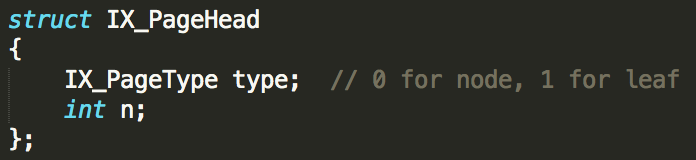
\includegraphics[width=4in]{Figures/IX_PageHead.png}
\end{figure}

type表示该页是中间节点还是叶子节点,n表示该页当前有的索引项个数。

中间节点页与叶子节点页的数据结构是相同的,如下图所示。
\begin{figure}[H]
\centering
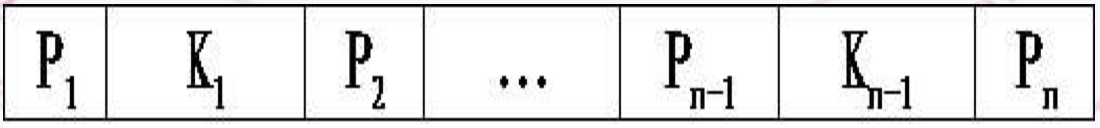
\includegraphics[width=4in]{Figures/indexstruct.png}
\end{figure}

其中P为指针,K为索引码值。区别在于,如果是中间节点,指针指向子节点(索引文件内的一个页),即P存储的是本文件的一个RID;如果是叶子节点,每个索引码值对应一条数据记录,P存储的是该记录在数据表页中的RID;叶子节点最后一个索引码值后面的指针P指向后面一个叶子节点,这样一个索引文件中存储的所有索引项按顺序可以形成一个列表。

索引的插入、删除、查询等功能按照B+树的要求实现。

索引模块的实现仿照记录管理模块,主要包括3个类,即 IX\_Manager、IX\_IndexHandle 以及 IX\_IndexScan。

\begin{figure}[H]
\centering
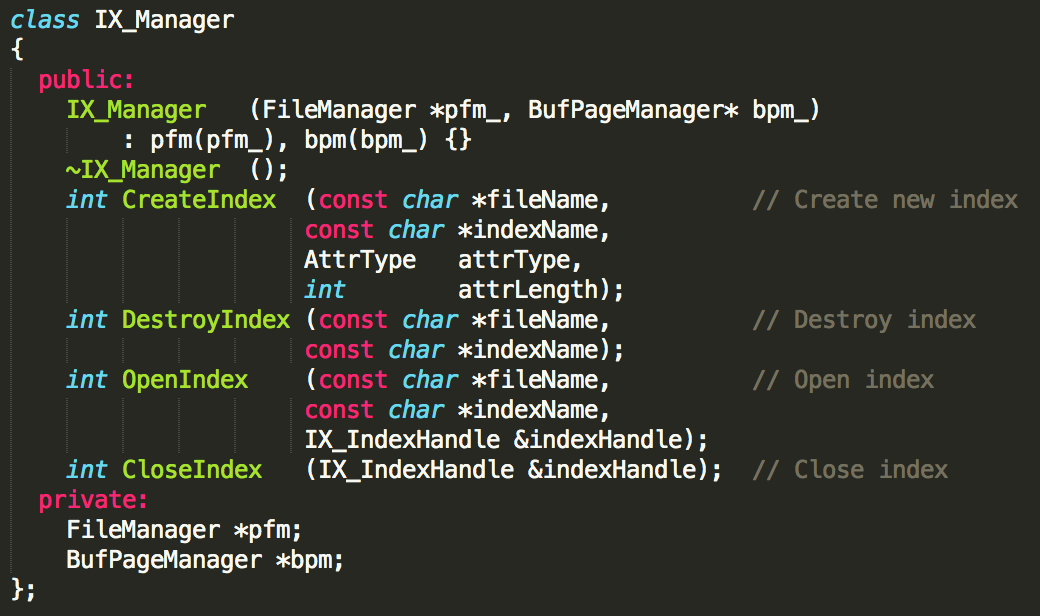
\includegraphics[width=4.5in]{Figures/IX_Manager.png}
\end{figure}

IX\_Manager提供的接口包括新建索引、打开索引、关闭索引和删除索引。

\begin{figure}[H]
\centering
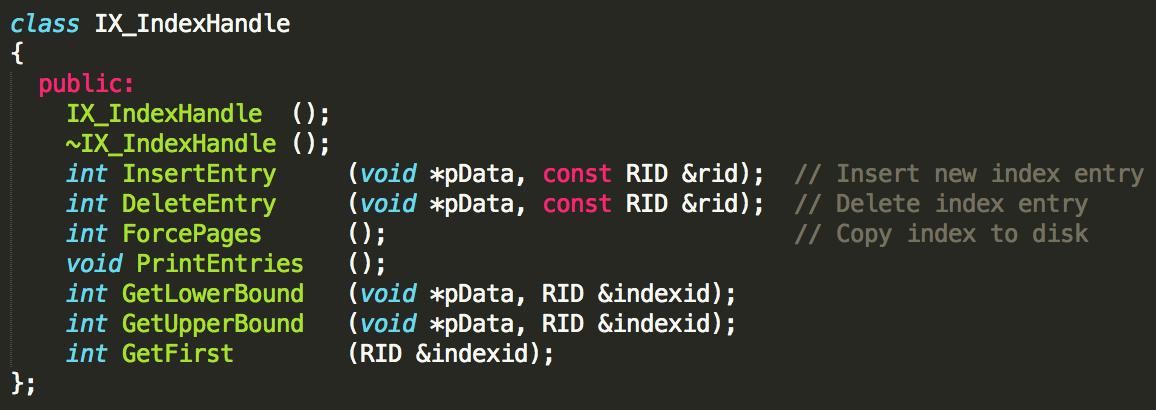
\includegraphics[width=5.5in]{Figures/IX_IndexHandle.png}
\end{figure}

IX\_IndexHandle提供的接口包括插入索引项、删除索引项,以及为了支持查询提供首项、LowerBound和UpperBound的查询。B+树的主要功能实现在这个类中完成。

\begin{figure}[H]
\centering
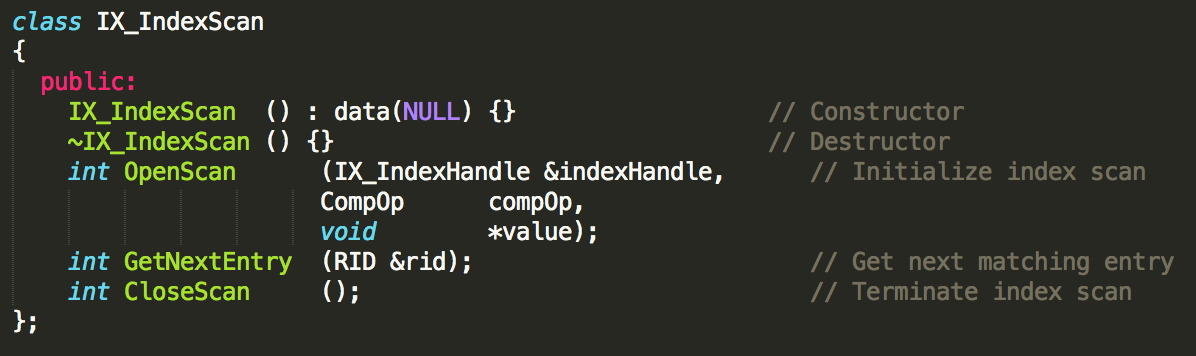
\includegraphics[width=5.5in]{Figures/IX_IndexScan.png}
\end{figure}

IX\_IndexScan提供的接口和RM\_FileScan完全一致,区别在于IX\_IndexScan的查询操作是通过索引在B+树上完成的,效率更高。

其他的模块在执行新建索引以及插入、删除、更新记录的同时,要更新相关的索引。

\section{扩展功能}

\subsection{域完整性约束}
域完整性约束,即建表时有CHECK关键字,约束某一个属性可能的取值。

为实现这一功能,我们对每个有域完整性约束的属性,新建一个和索引文件一样的约束文件,命名方式为RelName.AttrName.check.index,也用IX\_Manager管理。在这个文件中,将该属性可能的取值作为索引项依次插入。

插入记录时,检查所有有域完整性约束的属性值是否在其约束文件中存在。如果存在,允许插入,否则拒绝并报错。

\subsection{外键约束}
外键约束,用于与另一张表的关联,以保持数据的一致性。外键一定是另一张表的主键,因此一定是建好索引
的。

所以,在更新一个有外键约束的记录时,打开关联表的主键索引,检查更新后的值是否存在。如果存在,允许更新,否则拒绝并报错。

\subsection{模糊匹配}

\subsection{三个表以上的连接}

\subsection{聚集查询}

\subsection{图形用户界面}
图形用户界面使用Qt实现,在文本框中输入SQL语句,点击后通过命令行执行,然后将输出的结果以表格形式显示。
